\documentclass{standalone}
\usepackage[utf8]{inputenc}
\usepackage{tikz}
\usepackage{color}
\usetikzlibrary{arrows,shapes,positioning,shadows,trees}

\tikzset{
  basic/.style  = {draw, text width=3cm, drop shadow, font=\sffamily, rectangle},
  root/.style   = {basic, rounded corners=2pt, thin, align=center,
                   fill=yellow!60},
  level 2/.style = {basic, rounded corners=6pt, thin,align=center, fill=yellow!40,
                   text width=12em},
  level 3/.style = {basic, rounded corners=6pt, thin,align=center, fill=yellow!40,
                   text width=8em},
  level 4/.style = {basic, thin, align=left, fill=yellow!20, text width=8em}
}

\begin{document}

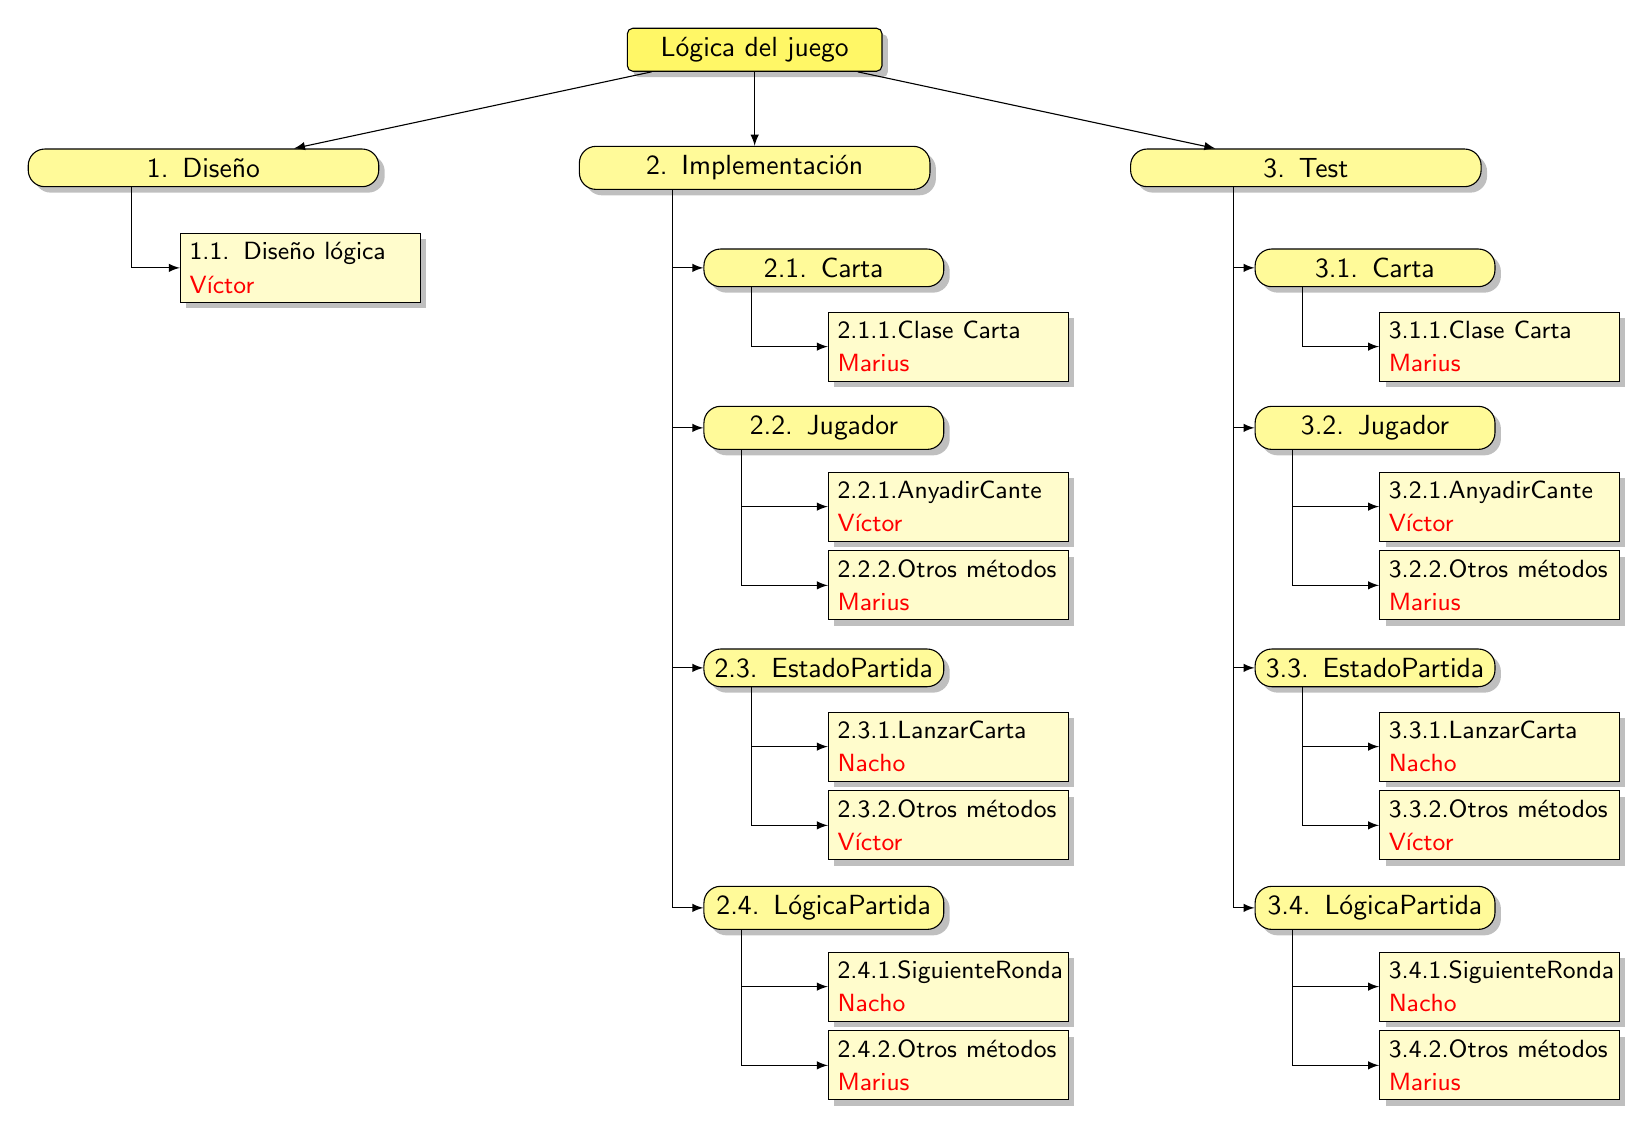
\begin{tikzpicture}[
  level 1/.style={sibling distance=70mm},
  edge from parent/.style={->,draw},
  >=latex]

% raiz inicial
\node[root] {Lógica del juego}
% The first level, as children of the initial tree
  child {node[level 2] (c1) {1. Diseño}}
  child {node[level 2] (c2) {2. Implementación}}
  child {node[level 2] (c3) {3. Test}};

\begin{scope}[every node/.style={level 3}]
\node [below of = c2, xshift=25pt, node distance=0.5in] (c21) {2.1. Carta};
\node [below of = c21, node distance=0.8in] (c22) {2.2. Jugador};
\node [below of = c22, node distance=1.2in] (c23) {2.3. EstadoPartida};
\node [below of = c23, node distance=1.2in] (c24) {2.4. LógicaPartida};
\end{scope}

\begin{scope}[every node/.style={level 3}]
\node [below of = c3, xshift=25pt, node distance=0.5in] (c31) {3.1. Carta};
\node [below of = c31, node distance=0.8in] (c32) {3.2. Jugador};
\node [below of = c32, node distance=1.2in] (c33) {3.3. EstadoPartida};
\node [below of = c33, node distance=1.2in] (c34) {3.4. LógicaPartida};
\end{scope}

% The second level, relatively positioned nodes
\begin{scope}[every node/.style={level 4}]
\node [below of = c1,node distance=0.5in, xshift=35pt] (c11) {\small{1.1. Diseño lógica} \\ \textcolor{red}{\small{Víctor}}};

\node [below of = c21, xshift=45pt] (c211) {\small{2.1.1.Clase Carta} \\ \textcolor{red}{\small{Marius}}};

\node [below of = c22, xshift=45pt] (c221) {\small{2.2.1.AnyadirCante} \\ \textcolor{red}{\small{Víctor}}};
\node [below of = c221] (c222) {\small{2.2.2.Otros métodos} \\ \textcolor{red}{\small{Marius}}};

\node [below of = c23, xshift=45pt] (c231) {\small{2.3.1.LanzarCarta} \\ \textcolor{red}{\small{Nacho}}};
\node [below of = c231] (c232) {\small{2.3.2.Otros métodos} \\ \textcolor{red}{\small{Víctor}}};

\node [below of = c24, xshift=45pt] (c241) {\small{2.4.1.SiguienteRonda} \\ \textcolor{red}{\small{Nacho}}};
\node [below of = c241] (c242) {\small{2.4.2.Otros métodos} \\ \textcolor{red}{\small{Marius}}};

\node [below of = c31, xshift=45pt] (c311) {\small{3.1.1.Clase Carta} \\ \textcolor{red}{\small{Marius}}};

\node [below of = c32, xshift=45pt] (c321) {\small{3.2.1.AnyadirCante} \\ \textcolor{red}{\small{Víctor}}};
\node [below of = c321] (c322) {\small{3.2.2.Otros métodos} \\ \textcolor{red}{\small{Marius}}};

\node [below of = c33, xshift=45pt] (c331) {\small{3.3.1.LanzarCarta} \\ \textcolor{red}{\small{Nacho}}};
\node [below of = c331] (c332) {\small{3.3.2.Otros métodos} \\ \textcolor{red}{\small{Víctor}}};

\node [below of = c34, xshift=45pt] (c341) {\small{3.4.1.SiguienteRonda} \\ \textcolor{red}{\small{Nacho}}};
\node [below of = c341] (c342) {\small{3.4.2.Otros métodos} \\ \textcolor{red}{\small{Marius}}};

\end{scope}

\foreach \value in {1,2,3,4}
  \draw [->] (c2.195) |- (c2\value.west);

\foreach \value in {1,2,3,4}
  \draw [->] (c3.195) |- (c3\value.west);

\foreach \value in {1}
  \draw[->] (c1.195) |- (c1\value.west);

\foreach \value in {1}
  \draw[->] (c21.195) |- (c21\value.west);

\foreach \value in {1,2}
  \draw[->] (c22.195) |- (c22\value.west);

\foreach \value in {1,2}
  \draw[->] (c23.195) |- (c23\value.west);

\foreach \value in {1,2}
  \draw[->] (c24.195) |- (c24\value.west);

\foreach \value in {1}
  \draw[->] (c31.195) |- (c31\value.west);

\foreach \value in {1,2}
  \draw[->] (c32.195) |- (c32\value.west);

\foreach \value in {1,2}
  \draw[->] (c33.195) |- (c33\value.west);

\foreach \value in {1,2}
  \draw[->] (c34.195) |- (c34\value.west);

\end{tikzpicture}

\end{document}
